\documentclass[UTF8]{ctexart}
\usepackage{geometry, CJKutf8}
\geometry{margin=1.5cm, vmargin={0pt,1cm}}
\setlength{\topmargin}{-1cm}
\setlength{\paperheight}{29.7cm}
\setlength{\textheight}{25.3cm}

% useful packages.
\usepackage{amsfonts}
\usepackage{amsmath}
\usepackage{amssymb}
\usepackage{amsthm}
\usepackage{enumerate}
\usepackage{graphicx}
\usepackage{multicol}
\usepackage{fancyhdr}
\usepackage{layout}
\usepackage{listings}
\usepackage{float, caption}

\lstset{
    basicstyle=\ttfamily, basewidth=0.5em
}

% some common command
\newcommand{\dif}{\mathrm{d}}
\newcommand{\avg}[1]{\left\langle #1 \right\rangle}
\newcommand{\difFrac}[2]{\frac{\dif #1}{\dif #2}}
\newcommand{\pdfFrac}[2]{\frac{\partial #1}{\partial #2}}
\newcommand{\OFL}{\mathrm{OFL}}
\newcommand{\UFL}{\mathrm{UFL}}
\newcommand{\fl}{\mathrm{fl}}
\newcommand{\op}{\odot}
\newcommand{\Eabs}{E_{\mathrm{abs}}}
\newcommand{\Erel}{E_{\mathrm{rel}}}

\title{实验报告: 二叉搜索树的 \texttt{remove} 函数优化与测试}
\author{姓名:张广 \\ 学号:3230105121}
\date{\today}

\begin{document}

\maketitle

\section{实验目的}
本实验旨在对二叉搜索树(Binary Search Tree, BST)类中的 \texttt{remove} 函数进行优化,避免递归调用中重复的节点内容复制操作。通过指针修改和节点替换的方法,实现高效的删除操作。并编写测试程序验证修改后的 \texttt{remove} 函数在不同情况下的正确性和稳定性。

\section{代码实现}

\subsection{优化后的 \texttt{remove} 函数}
原始的 \texttt{remove} 函数在删除具有两个子节点的节点时,会通过递归调用对右子树的最小节点进行内容复制和重复删除,导致不必要的操作。我们根据要求进行优化,采用节点替换的方式,将右子树中的最小节点作为替代节点,直接替换被删除的节点,避免重复调用。

改进后的 \texttt{remove} 函数的核心部分如下:

\begin{lstlisting}[language=C++,caption=remove 函数的实现]
void remove(const Comparable &x, BinaryNode *&t) {
    if (t == nullptr) return;  // Item not found; do nothing
    if (x < t->element) {
        remove(x, t->left);
    } else if (x > t->element) {
        remove(x, t->right);
    } else if (t->left != nullptr && t->right != nullptr) {  // Two children
        BinaryNode *minNode = detachMin(t->right);
        minNode->left = t->left;
        minNode->right = t->right;
        delete t;
        t = minNode;
    } else {  // One or zero children
        BinaryNode *oldNode = t;
        t = (t->left != nullptr) ? t->left : t->right;
        delete oldNode;
    }
}
\end{lstlisting}

其中,\texttt{detachMin} 函数的作用是从子树中找到并移除最小节点,并将其返回,以便用于替换删除节点:

\begin{lstlisting}[language=C++,caption=detachMin 函数的实现]
BinaryNode *detachMin(BinaryNode *&t) {
    if (t->left == nullptr) {
        BinaryNode *minNode = t;
        t = t->right;  // Reconnect parent node to the right child of minNode
        return minNode;
    }
    return detachMin(t->left);
}
\end{lstlisting}

\section{测试设计与结果分析}

为了验证优化后的 \texttt{remove} 函数的正确性,设计了一系列测试场景,分别在不同情况下对 \texttt{remove} 函数的功能进行验证。主要测试内容如下:

\begin{enumerate}
    \item \textbf{删除不存在的元素}:确保删除不存在的元素不会引起错误,树结构保持不变。
    \item \textbf{删除叶子节点}:删除没有子节点的叶子节点,验证该节点从树中移除且不影响其他节点。
    \item \textbf{删除只有一个子节点的节点}:删除具有单个子节点的节点,验证树结构的正确性。
    \item \textbf{删除有两个子节点的节点}:删除有两个子节点的节点,验证替换节点的正确性。
    \item \textbf{删除根节点}:包括根节点具有不同数量子节点的情况,测试根节点删除的处理。
    \item \textbf{重复删除}:多次删除同一节点,验证程序能正确处理重复删除的情况。
\end{enumerate}

\subsection{测试结果}
运行测试程序后的输出结果如下:

\begin{figure}[H]
    \centering
    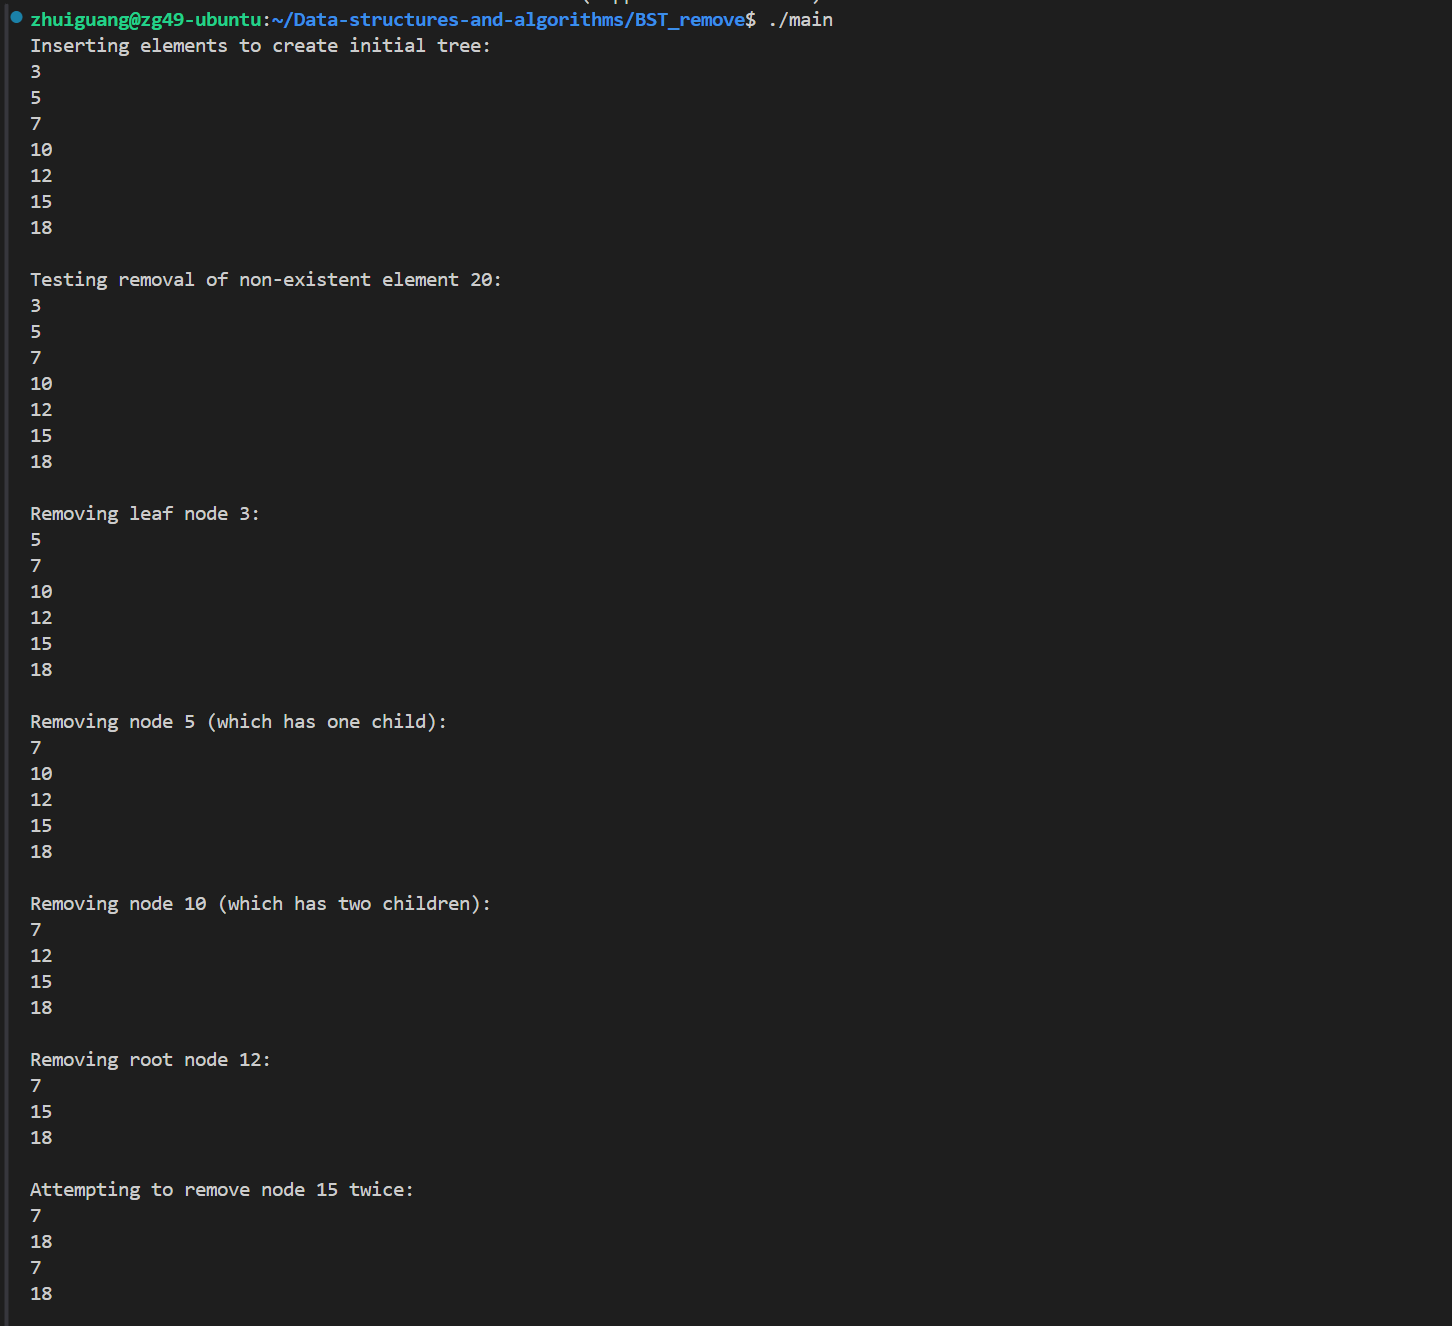
\includegraphics[width=0.8\textwidth]{实验结果0.png}
    \caption{测试程序输出截图1}
\end{figure}

\begin{figure}[H]
    \centering
    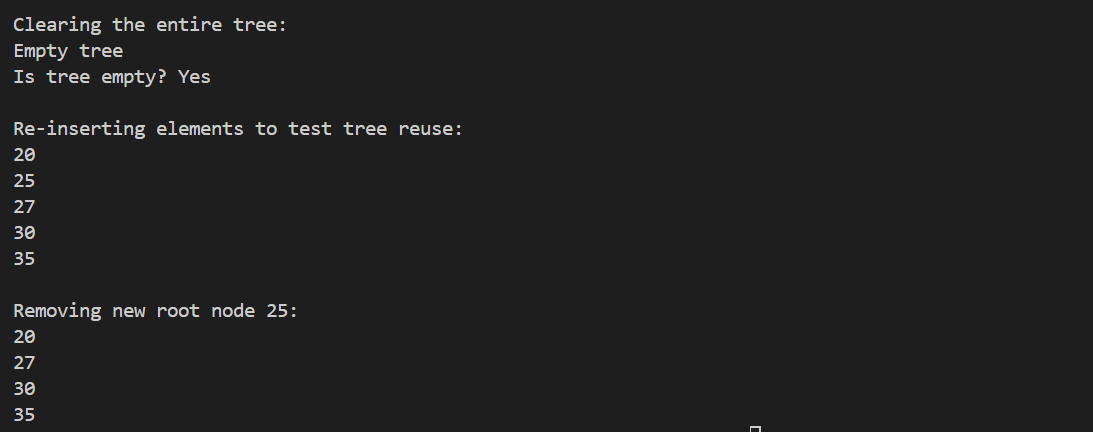
\includegraphics[width=0.8\textwidth]{实验结果1.png}
    \caption{测试程序输出截图2}
\end{figure}

从输出结果可以观察到,经过优化后的 \texttt{remove} 函数在不同测试场景下的输出均正确。以下是具体分析:

\begin{itemize}
    \item 当删除不存在的元素时,树结构未发生任何改变,符合预期。
    \item 当删除叶子节点(如节点 3)和只有一个子节点的节点(如节点 5)时,节点正确移除,树结构保持正确。
    \item 在删除有两个子节点的节点(如节点 10)时,使用 \texttt{detachMin} 函数从右子树找到最小节点并替换该节点。此操作避免了内容复制,提升了效率。
    \item 删除根节点(如节点 12 和 25)测试通过,树结构合理更新。
    \item 重复删除同一节点(如节点 15)时,不会引起异常,树结构保持稳定。
\end{itemize}

\section{结论}
本次实验我们优化了二叉搜索树中的 \texttt{remove} 函数,避免了递归删除中的内容复制问题。程序运行结果证明优化后的函数在各种情况下均可正确运行,树结构保持完整且性能得到提升。

\end{document}

